\documentclass[a4paper, UTF-8]{article}
\usepackage{algorithm}
\usepackage{algpseudocode}
\usepackage{amsmath}
\usepackage{amsfonts}
\usepackage{amsthm}
\usepackage{tikz}
\usetikzlibrary{automata, positioning, arrows}
\usepackage[utf8]{inputenc} % allow utf-8 input
\usepackage[T1]{fontenc}    % use 8-bit T1 fonts
\usepackage{hyperref}       % hyperlinks
\usepackage{url}            % simple URL typesetting
\usepackage{booktabs}       % professional-quality tables
\usepackage{amsfonts}       % blackboard math symbols
\usepackage{nicefrac}       % compact symbols for 1/2, etc.
\usepackage{microtype}      % microtypography
\usepackage{xcolor}         % colors

\theoremstyle{plain}
\newtheorem{theorem}{\indent Theorem}[section]
\newtheorem{lemma}[theorem]{\indent Lemma}
\newtheorem{assumption}{\indent Assumption}[section]
\newtheorem{note}[theorem]{\indent Notation}
\newtheorem{proposition}[theorem]{\indent Proposition}
\newtheorem{corollary}[theorem]{\indent Corollary}
\newtheorem{definition}{\indent Definition}[section]
\newtheorem{example}{\indent Example}[section]
\newtheorem{remark}{\indent Remark}[section]
\newenvironment{solution}{\begin{proof}[\indent\bf Solution]}{\end{proof}}
\renewcommand{\proofname}{\indent\bf Proof}

\begin{document}

\title{\bf{Lab2 Answers}}

\author{Yanqiao Chen*\\ 
  Department of Computer Science and Engineering\\
  Southern University of Science and Technology\\
  \texttt{12412115@mail.sustech.edu.cn}
  }

\maketitle

\section{Question 1}

\subsection{a) $\{w|w \text{ ends with } $00$\}$} 

\begin{center} 
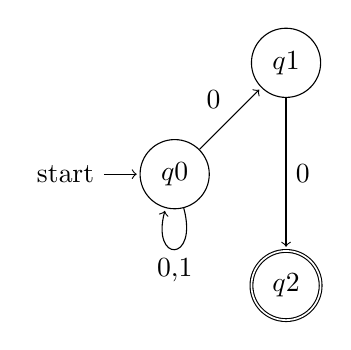
\begin{tikzpicture}[shorten >=1pt, node distance=2cm, on grid, auto] 
   \node[state, initial] (q_0)   {$q0$}; 
   \node[state] (q_1) [above right=of q_0] {$q1$}; 
   \node[state, accepting] (q_2) [below right=of q_0] {$q2$}; 
   \path[->] 
    (q_0) edge  node {0} (q_1)
    (q_0) edge [loop below] node {0,1} (q_0)
    (q_1) edge  node {0} (q_2)
    ;
\end{tikzpicture}
\end{center}


\subsection{b) $\{w| w \text{ contains the substring } 0101\}$}

\begin{center} 
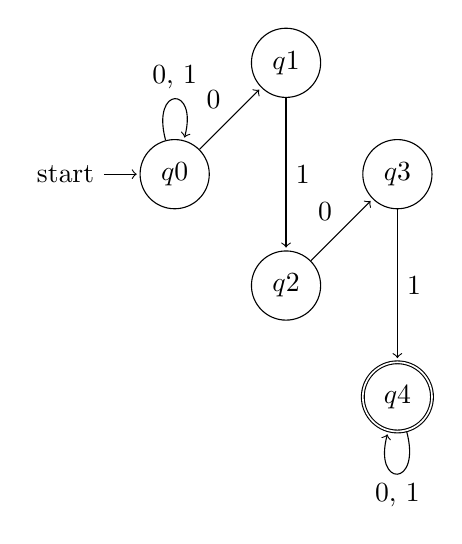
\begin{tikzpicture}[shorten >=1pt, node distance=2cm, on grid, auto] 
   \node[state, initial] (q_0)   {$q0$}; 
   \node[state] (q_1) [above right=of q_0] {$q1$}; 
   \node[state] (q_2) [below right=of q_0] {$q2$}; 
   \node[state] (q_3) [below right=of q_1] {$q3$}; 
   \node[state, accepting] (q_4) [below right=of q_2] {$q4$};
   \path[->] 
    (q_0) edge  node {0} (q_1)
    (q_1) edge node {1} (q_2)
    (q_2) edge node {0} (q_3)
    (q_3) edge node {1} (q_4)
    (q_0) edge [loop above] node {0, 1} (q_0)
    (q_4) edge [loop below] node {0, 1} (q_4)
    ;
\end{tikzpicture}
\end{center}

\subsection{c) $\{w| w \text{ contains an even number of } 0\text{'s, or contains exactly two 1's}\}$}

\begin{center} 
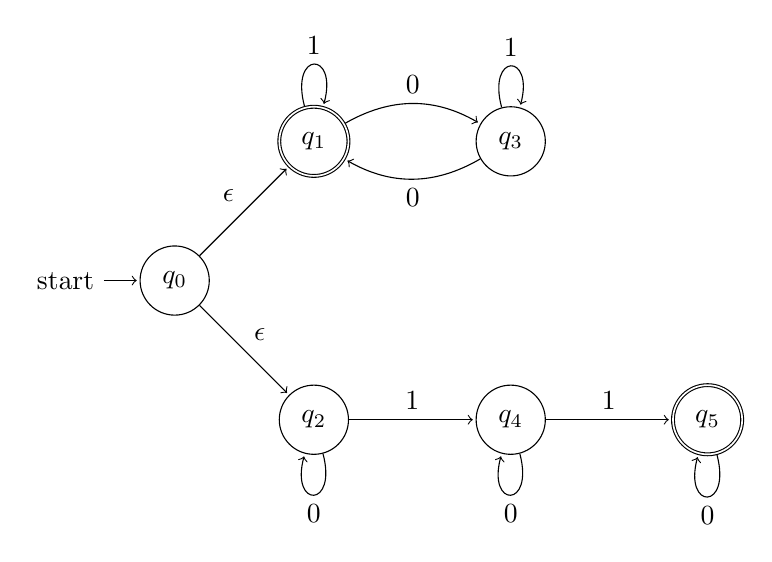
\begin{tikzpicture}[shorten >=1pt, node distance=2.5cm, on grid, auto] 
   \node[state, initial] (q_0)   {$q_0$}; 
   
   % 偶数个 0 分支 (q1, q3)
   \node[state, accepting] (q_1) [above right=of q_0] {$q_1$}; 
   \node[state] (q_3) [right=of q_1] {$q_3$}; 
   
   % 恰好两个 1 分支 (q2, q4, q5)
   \node[state] (q_2) [below right=of q_0] {$q_2$}; 
   \node[state] (q_4) [right=of q_2] {$q_4$};
   \node[state, accepting] (q_5) [right=of q_4] {$q_5$};
   
   \path[->] 
    % 从初始状态分支
    (q_0) edge  node {$\epsilon$} (q_1)
    (q_0) edge  node {$\epsilon$} (q_2)
    
    % 偶数个 0：q1(偶数,接受) <-> q3(奇数)
    (q_1) edge [bend left] node {0} (q_3)
    (q_3) edge [bend left] node {0} (q_1)
    (q_1) edge [loop above] node {1} (q_1)
    (q_3) edge [loop above] node {1} (q_3)
    
    % 恰好两个 1：q2(0个1) -> q4(1个1) -> q5(2个1,接受)
    (q_2) edge node {1} (q_4)
    (q_4) edge node {1} (q_5)
    (q_2) edge [loop below] node {0} (q_2)
    (q_4) edge [loop below] node {0} (q_4)
    (q_5) edge [loop below] node {0} (q_5)
    ;
\end{tikzpicture}
\end{center}

\subsection{d) Language $\{0\}$}


\begin{center} 
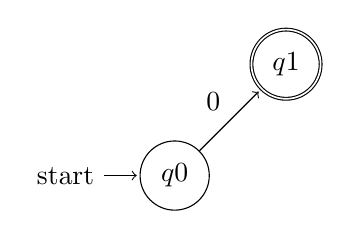
\begin{tikzpicture}[shorten >=1pt, node distance=2cm, on grid, auto] 
   \node[state, initial] (q_0)   {$q0$}; 
   \node[state, accepting] (q_1) [above right=of q_0] {$q1$}; 
   \path[->] 
    (q_0) edge  node {0} (q_1)
    ;
\end{tikzpicture}
\end{center}

\subsection{e) The language $0^*1^*0^+$ using three states}

\begin{center} 
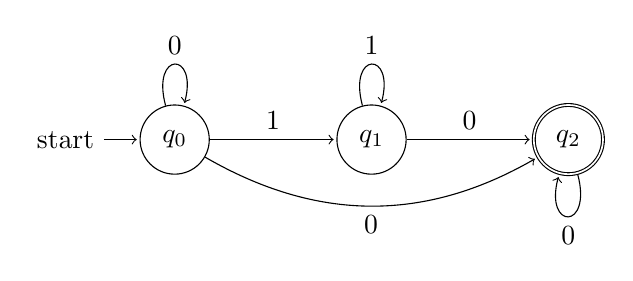
\begin{tikzpicture}[shorten >=1pt, node distance=2.5cm, on grid, auto] 
   \node[state, initial] (q_0)   {$q_0$}; 
   \node[state] (q_1) [right=of q_0] {$q_1$}; 
   \node[state, accepting] (q_2) [right=of q_1] {$q_2$}; 
   
   \path[->] 
    % q_0 的自环 (0*)
    (q_0) edge [loop above] node {0} (q_0)
    % q_0 到 q_1 (进入 1*)
    (q_0) edge node {1} (q_1)
    % q_0 到 q_2 (开始结尾的 0+)
    (q_0) edge [bend right=30] node[below] {0} (q_2)
    
    % q_1 的自环 (1*)
    (q_1) edge [loop above] node {1} (q_1)
    % q_1 到 q_2 (进入结尾的 0+)
    (q_1) edge node {0} (q_2)
    
    % q_2 的自环 (0+)
    (q_2) edge [loop below] node {0} (q_2)
    ;
\end{tikzpicture}
\end{center}

\subsection{f) The language $1^*(001^+)^*$ with three states}

\begin{center} 
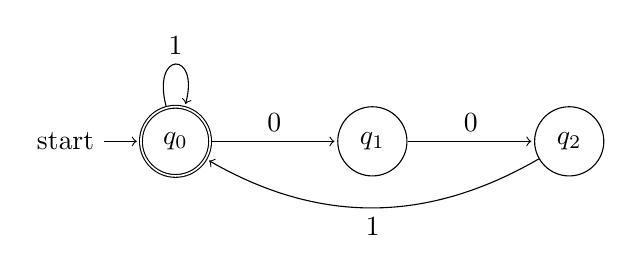
\begin{tikzpicture}[shorten >=1pt, node distance=2.5cm, on grid, auto] 
   \node[state, initial, accepting] (q_0)   {$q_0$}; 
   \node[state] (q_1) [right=of q_0] {$q_1$}; 
   \node[state] (q_2) [right=of q_1] {$q_2$}; 
   
   \path[->] 
    % q_0: 处理开头的 1*，也是 $(001^+)^*$ 每个循环的结束点
    (q_0) edge [loop above] node {1} (q_0)
    (q_0) edge node {0} (q_1)
    
    % q_1: 等待第二个 0 完成 "00"
    (q_1) edge node {0} (q_2)
    
    % q_2: 完成 00，必须读至少一个 1 回到 q_0
    (q_2) edge [bend left=30] node {1} (q_0)
    ;
\end{tikzpicture}
\end{center}

\subsection{g) Language $\{\epsilon\}$}

\begin{center} 
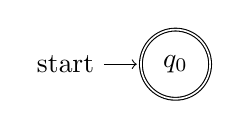
\begin{tikzpicture}[shorten >=1pt, node distance=2.5cm, on grid, auto] 
   \node[state, initial, accepting] (q_0)   {$q_0$}; 
    ;
\end{tikzpicture}
\end{center}

\subsection{h) Language $\{0^*\}$}

\begin{center} 
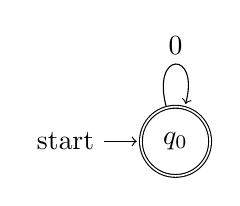
\begin{tikzpicture}[shorten >=1pt, node distance=2.5cm, on grid, auto] 
   \node[state, initial, accepting] (q_0)   {$q_0$}; 
   \path[->] 
    (q_0) edge [loop above] node {0} (q_0)
    ;
\end{tikzpicture}
\end{center}

\section{Question 2} 

\subsection{a} 

\begin{center} 
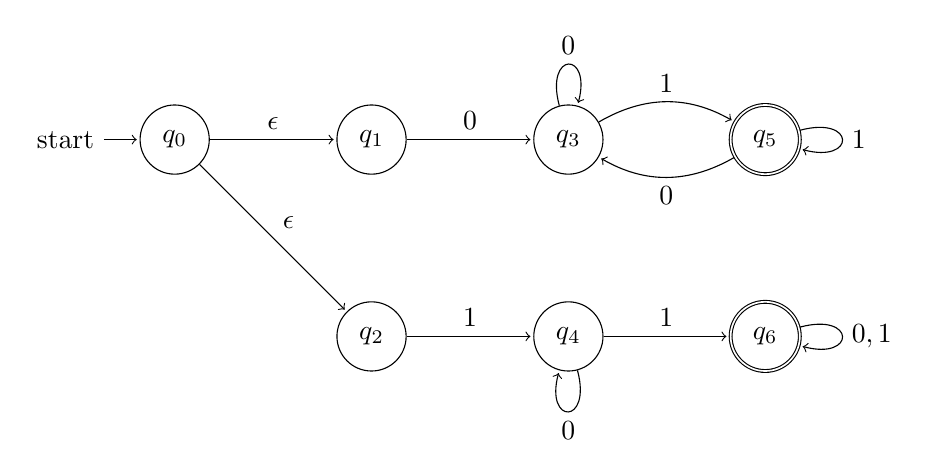
\begin{tikzpicture}[shorten >=1pt, node distance=2.5cm, on grid, auto] 
   \node[state, initial] (q_0) {$q_0$}; 
   \node[state] (q_1) [right=of q_0] {$q_1$}; 
   \node[state] (q_2) [below=of q_1] {$q_2$};
   \node[state] (q_3) [right of=q_1] {$q_3$}; 
   \node[state] (q_4) [right of=q_2] {$q_4$};
   \node[state, accepting] (q_5) [right=of q_3] {$q_5$};
   \node[state, accepting] (q_6) [right=of q_4] {$q_6$};
   \path[->] 
    (q_0) edge node {$\epsilon$} (q_1)
    (q_0) edge node {$\epsilon$} (q_2)
    (q_1) edge node {$0$} (q_3)
    (q_3) edge [bend left] node {$1$} (q_5) 
    (q_5) edge [loop right] node {$1$} (q_5)
    (q_3) edge [loop above] node {$0$} (q_3)
    (q_5) edge [bend left] node {$0$} (q_3)
    (q_2) edge node {$1$} (q_4)
    (q_4) edge node {$1$} (q_6)
    (q_4) edge [loop below] node {$0$} (q_4)
    (q_6) edge [loop right] node {$0, 1$} (q_6)
    ;
\end{tikzpicture}
\end{center}

\subsection{b}

\begin{center} 
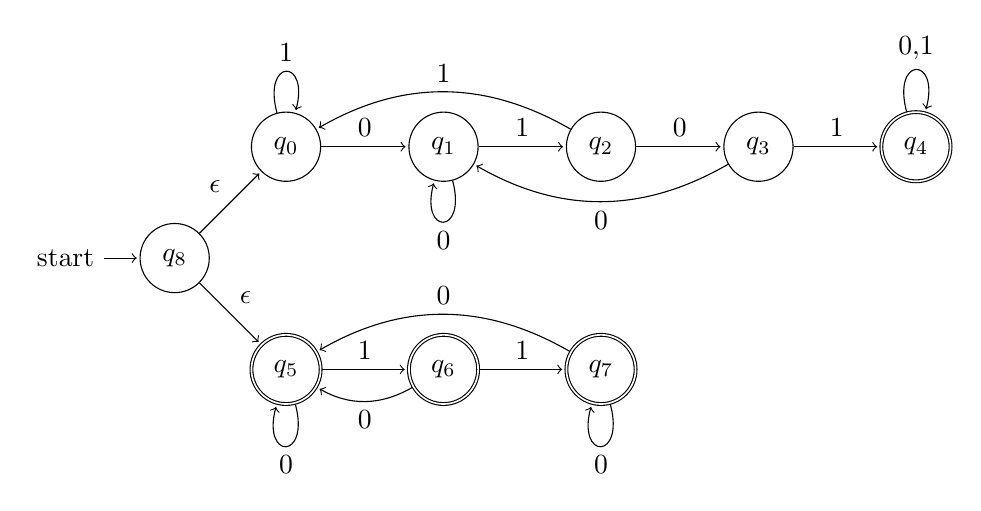
\begin{tikzpicture}[shorten >=1pt, node distance=2cm, on grid, auto] 
   % 新建初始状态
   \node[state, initial] (q_8) {$q_8$}; 
   
   % L1 部分 (0101)
   \node[state] (q_0) [above right=of q_8] {$q_0$}; 
   \node[state] (q_1) [right=of q_0] {$q_1$}; 
   \node[state] (q_2) [right=of q_1] {$q_2$};
   \node[state] (q_3) [right=of q_2] {$q_3$};
   \node[state, accepting] (q_4) [right=of q_3] {$q_4$};
   
   % L2 部分 (不含111)
   \node[state, accepting] (q_5) [below right=of q_8] {$q_5$};
   \node[state, accepting] (q_6) [right=of q_5] {$q_6$};
   \node[state, accepting] (q_7) [right=of q_6] {$q_7$};
   
   \path[->] 
    % 并集构造：从 q_8 分支
    (q_8) edge node {$\epsilon$} (q_0)
    (q_8) edge node {$\epsilon$} (q_5)
    
    % L1 转移 (找 0101)
    % q_0: 等待第一个0
    (q_0) edge [loop above] node {1} (q_0)
    (q_0) edge node {0} (q_1)
    % q_1: 已有0，等待1
    (q_1) edge [loop below] node {0} (q_1)
    (q_1) edge node {1} (q_2)
    % q_2: 已有01，等待0
    (q_2) edge node {0} (q_3)
    (q_2) edge [bend right=30] node[above] {1} (q_0)
    % q_3: 已有010，等待1
    (q_3) edge node {1} (q_4)
    (q_3) edge [bend left=30] node[below] {0} (q_1)
    % q_4: 接受状态
    (q_4) edge [loop above] node {0,1} (q_4)
    
    % L2 转移 (不含111)
    % 计数连续1的个数
    (q_5) edge [loop below] node {0} (q_5)
    (q_5) edge node {1} (q_6)
    (q_6) edge [bend left=30] node[below] {0} (q_5)
    (q_6) edge node {1} (q_7)
    (q_7) edge [bend right=30] node[above] {0} (q_5)
    (q_7) edge [loop below] node {0} (q_7)
    % q_7 读1会进入未定义状态（相当于陷阱），所以不写
    ;
\end{tikzpicture}
\end{center}

\section{Question 3}

\subsection{a) $L_1 = \{w \mid \text{the length of } w \text{ is at most 4}\}$, $L_2 = \{w \mid \text{every odd position of } w \text{ is a } 1\}$}


\begin{center}
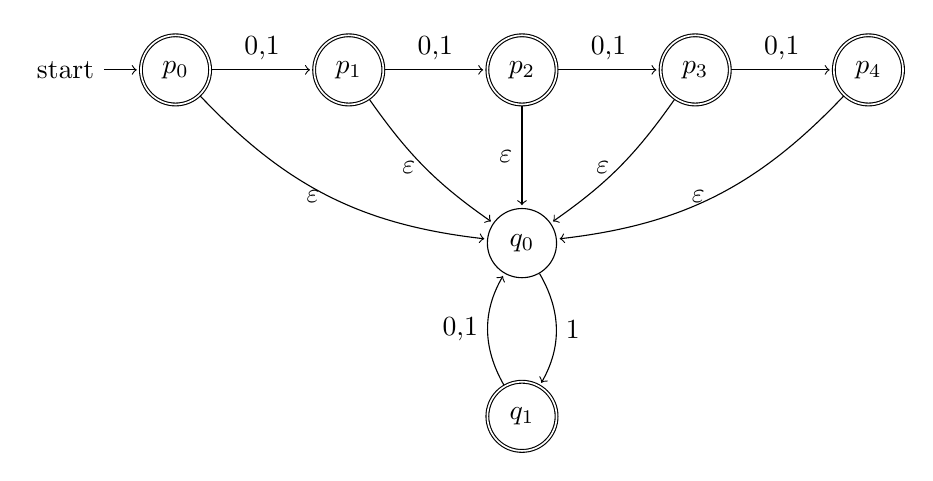
\begin{tikzpicture}[shorten >=1pt, node distance=2.2cm, on grid, auto]
   % M1 部分（长度计数）
   \node[state, initial, accepting] (p_0) {$p_0$};
   \node[state, accepting] (p_1) [right=of p_0] {$p_1$};
   \node[state, accepting] (p_2) [right=of p_1] {$p_2$};
   \node[state, accepting] (p_3) [right=of p_2] {$p_3$};
   \node[state, accepting] (p_4) [right=of p_3] {$p_4$};
   
   % M2 部分（奇偶位置）
   \node[state] (q_0) [below=of p_2] {$q_0$};
   \node[state, accepting] (q_1) [below=of q_0] {$q_1$};
   
   \path[->]
    % M1 的转移（长度计数）
    (p_0) edge node {0,1} (p_1)
    (p_1) edge node {0,1} (p_2)
    (p_2) edge node {0,1} (p_3)
    (p_3) edge node {0,1} (p_4)
    
    % epsilon 从 M1 的所有接受状态到 M2 的初始状态
    (p_0) edge [bend right=20] node[left] {$\varepsilon$} (q_0)
    (p_1) edge [bend right=10] node[left] {$\varepsilon$} (q_0)
    (p_2) edge node[left] {$\varepsilon$} (q_0)
    (p_3) edge [bend left=10] node[left] {$\varepsilon$} (q_0)
    (p_4) edge [bend left=20] node[left] {$\varepsilon$} (q_0)
    
    % M2 的转移（奇偶位置）
    % q_0: 奇数位置，只能读1，然后进入偶数位置q_1
    (q_0) edge [bend left] node {1} (q_1)
    % q_1: 偶数位置，可读0或1，然后回到奇数位置q_0
    (q_1) edge [bend left] node {0,1} (q_0)
    ;
\end{tikzpicture}
\end{center}


\subsection{b) $L_1 = \{w \mid w \text{ contains at least four 1s}\}$, $L_2 = \emptyset$}

\begin{center}
\begin{tikzpicture}[shorten >=1pt, node distance=2.2cm, on grid, auto]
   % M1 部分（计数1的个数）
   \node[state, initial] (p_0) {$p_0$};
   \node[state] (p_1) [right=of p_0] {$p_1$};
   \node[state] (p_2) [right=of p_1] {$p_2$};
   \node[state] (p_3) [right=of p_2] {$p_3$};
   \node[state] (p_4) [right=of p_3] {$p_4$};
   
   % M2 部分（空集 - 无接受状态）
   \node[state] (q_0) [below=of p_4] {$q_0$};
   
   \path[->]
    % M1 的转移
    (p_0) edge node {1} (p_1)
    (p_0) edge [loop above] node {0} (p_0)
    (p_1) edge node {1} (p_2)
    (p_1) edge [loop above] node {0} (p_1)
    (p_2) edge node {1} (p_3)
    (p_2) edge [loop above] node {0} (p_2)
    (p_3) edge node {1} (p_4)
    (p_3) edge [loop above] node {0} (p_3)
    (p_4) edge [loop above] node {0,1} (p_4)
    
    % epsilon 从 M1 的接受状态到 M2 的初始状态
    (p_4) edge node[left] {$\varepsilon$} (q_0)
    
    % M2 的转移（死状态）
    (q_0) edge [loop below] node {0,1} (q_0)
    ;
\end{tikzpicture}
\end{center}


\section{Question 4} 

\subsection{a) $L_1 = \{w \mid w \text{ contains at least four 1s}\}$}

\begin{center}
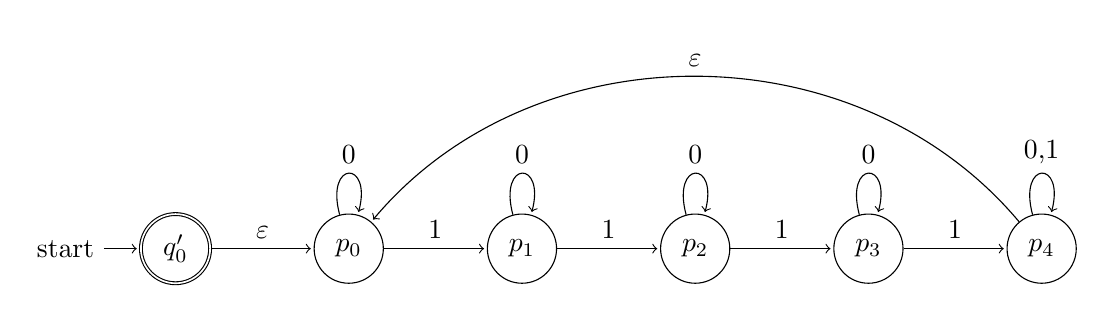
\begin{tikzpicture}[shorten >=1pt, node distance=2.2cm, on grid, auto]
   % 新的起始状态 q_0'
   \node[state, initial, accepting] (q0p) {$q_0'$};
   
   % 原自动机 M 部分
   \node[state] (p_0) [right=of q0p] {$p_0$};
   \node[state] (p_1) [right=of p_0] {$p_1$};
   \node[state] (p_2) [right=of p_1] {$p_2$};
   \node[state] (p_3) [right=of p_2] {$p_3$};
   \node[state] (p_4) [right=of p_3] {$p_4$};
   
   \path[->]
    % 从 q_0' 开始
    (q0p) edge node {$\varepsilon$} (p_0)
    
    % 原自动机的转移
    (p_0) edge node {1} (p_1)
    (p_0) edge [loop above] node {0} (p_0)
    (p_1) edge node {1} (p_2)
    (p_1) edge [loop above] node {0} (p_1)
    (p_2) edge node {1} (p_3)
    (p_2) edge [loop above] node {0} (p_2)
    (p_3) edge node {1} (p_4)
    (p_3) edge [loop above] node {0} (p_3)
    (p_4) edge [loop above] node {0,1} (p_4)
    
    % 接受状态回到原初始状态（实现Star）
    (p_4) edge [bend right=50] node[above] {$\varepsilon$} (p_0)
    ;
\end{tikzpicture}
\end{center}

\subsection{b) $L_1 = \{w \mid w \text{ contains at least two 1s and at most one 0}\}$}

\begin{center}
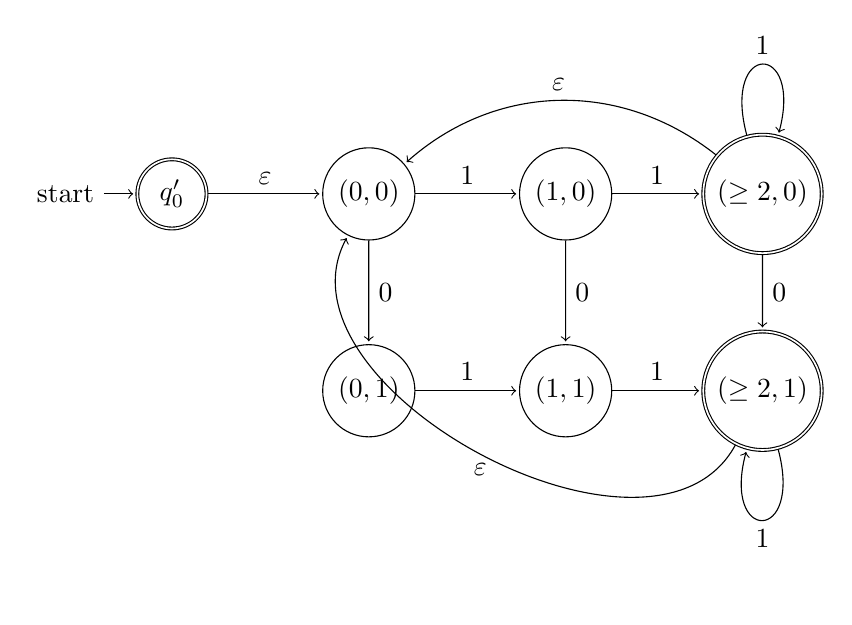
\begin{tikzpicture}[shorten >=1pt, node distance=2.5cm, on grid, auto, scale=0.9]
   % 新的起始状态 q_0'
   \node[state, initial, accepting] (q0p) {$q_0'$};
   
   % 原自动机：跟踪 (1的个数, 0的个数)
   % 第0行：0个0
   \node[state] (s00) [right=of q0p] {$(0,0)$};
   \node[state] (s10) [right=of s00] {$(1,0)$};
   \node[state, accepting] (s20) [right=of s10] {$(\geq 2,0)$};
   
   % 第1行：1个0
   \node[state] (s01) [below=of s00] {$(0,1)$};
   \node[state] (s11) [below=of s10] {$(1,1)$};
   \node[state, accepting] (s21) [below=of s20] {$(\geq 2,1)$};
   
   \path[->]
    % 从 q_0' 开始
    (q0p) edge node {$\varepsilon$} (s00)
    
    % 第0行转移（0个0）
    (s00) edge node {1} (s10)
    (s00) edge node {0} (s01)
    (s10) edge node {1} (s20)
    (s10) edge node {0} (s11)
    (s20) edge [loop above] node {1} (s20)
    (s20) edge node {0} (s21)
    
    % 第1行转移（1个0）
    (s01) edge node {1} (s11)
    (s11) edge node {1} (s21)
    (s21) edge [loop below] node {1} (s21)
    
    
    % 接受状态回到原初始状态（实现Star）
    (s20) edge [bend right=40] node[above] {$\varepsilon$} (s00)
    (s21) edge [bend left=90] node[below] {$\varepsilon$} (s00)
    ;
\end{tikzpicture}
\end{center}

\subsection{c) $L_1 = \emptyset$}

\begin{center}
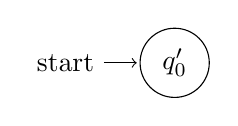
\begin{tikzpicture}[shorten >=1pt, node distance=2cm, on grid, auto]
   \node[state, initial] (q0p) {$q_0'$};
\end{tikzpicture}
\end{center}

\section{Question 5} 

\begin{proof}
Let the NFA be $M = (Q, \Sigma, \delta, q_0, F)$. We construct an equivalent NFA 
$M' = (Q', \Sigma, \delta', q_0, \{q_a\})$ with a single accept state as follows:

\begin{itemize}
    \item Add a new state $q_a \notin Q$ as the single accept state
    \item $Q' = Q \cup \{q_a\}$
    \item $\delta'$ includes all transitions in $\delta$, plus $\varepsilon$-transitions 
          from each original accept state to $q_a$:
          $$\delta'(f, \varepsilon) = \delta(f, \varepsilon) \cup \{q_a\} \quad \text{for all } f \in F$$
    \item For all other cases, $\delta'$ behaves the same as $\delta$
\end{itemize}

The new NFA $M'$ accepts a string $w$ if and only if there exists a path from $q_0$ 
to some $f \in F$ labeled by $w$ in $M$, followed by an $\varepsilon$-transition to $q_a$. 
Thus $L(M') = L(M)$.
\end{proof}

\section{Question 6}

\subsection{a)}

Let the $Q = \{\emptyset, \{1\}, \{2\}, \{1, 2\}\}$, $\Sigma = \{a, b\}$, $q_0 = \{1\}$, $F = \{\{1\}, \{1, 2\}\}$, and the delta be 

\begin{center}
\begin{tabular}{c|c|c}
    $\delta$ & $a$ & $b$ \\
    \hline
    $\emptyset$ & $\emptyset$ & $\emptyset$ \\
    $\{1\}$ & $\{1, 2\}$ & $\{2\}$ \\
    $\{2\}$ & $\emptyset$ & $\{1\}$ \\
    $\{1, 2\}$ & $\{1, 2\}$ & $\{1, 2\}$ \\
\end{tabular}
\end{center}

\subsection{b)}

Let $Q = \{\emptyset, \{1\}, \{2\}, \{3\}, \{1, 2\}, \{1, 3\}, \{2, 3\}, \{1, 2, 3\}\}$, $\Sigma = \{a, b\}$, $q_0 = \{1, 2\}$ (the $\varepsilon$-closure of $\{1\}$), $F = \{\{2\}, \{1, 2\}, \{2, 3\}, \{1, 2, 3\}\}$, and the delta be

\begin{center}
\begin{tabular}{c|c|c}
    $\delta$ & $a$ & $b$ \\
    \hline
    $\emptyset$ & $\emptyset$ & $\emptyset$ \\
    $\{1\}$ & $\{3\}$ & $\emptyset$ \\
    $\{2\}$ & $\{1, 2\}$ & $\emptyset$ \\
    $\{3\}$ & $\{2\}$ & $\{2, 3\}$ \\
    $\{1, 2\}$ & $\{1, 2, 3\}$ & $\emptyset$ \\
    $\{1, 3\}$ & $\{2, 3\}$ & $\{2, 3\}$ \\
    $\{2, 3\}$ & $\{1, 2\}$ & $\{2, 3\}$ \\
    $\{1, 2, 3\}$ & $\{1, 2, 3\}$ & $\{2, 3\}$ \\
\end{tabular}
\end{center}


\section{Question 7}

The complement of the language is $\{w| w \text{ contain a pair of 1s that are separated}$
$\text{ by an odd number of symbols}\}$ over $\Sigma = \{0, 1\}$. 

We construct a NFA for the complement language as follows:
\begin{center}
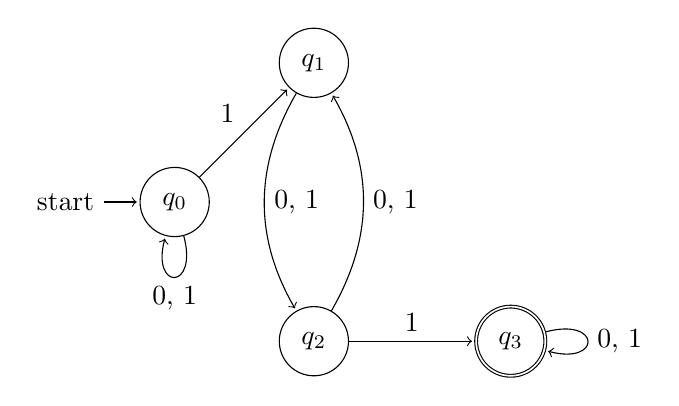
\begin{tikzpicture}[shorten >=1pt, node distance=2.5cm, on grid, auto]
   \node[state, initial] (q_0) {$q_0$};
   \node[state] (q_1) [above right=of q_0] {$q_1$};
   \node[state] (q_2) [below right=of q_0] {$q_2$};
   \node[state, accepting] (q_3) [right=of q_2] {$q_3$};
   
   \path[->]
   (q_0) edge node {1} (q_1)
   (q_0) edge [loop below] node {0, 1} (q_0)
   (q_1) edge [bend right]node {0, 1} (q_2)
   (q_2) edge node {1} (q_3)
   (q_2) edge [bend right] node [right]{0, 1} (q_1) 
   (q_3) edge [loop right] node {0, 1} (q_3)
    ;
\end{tikzpicture}
\end{center}

Thus, the corresponding NFA for the original language is: 

\begin{center}
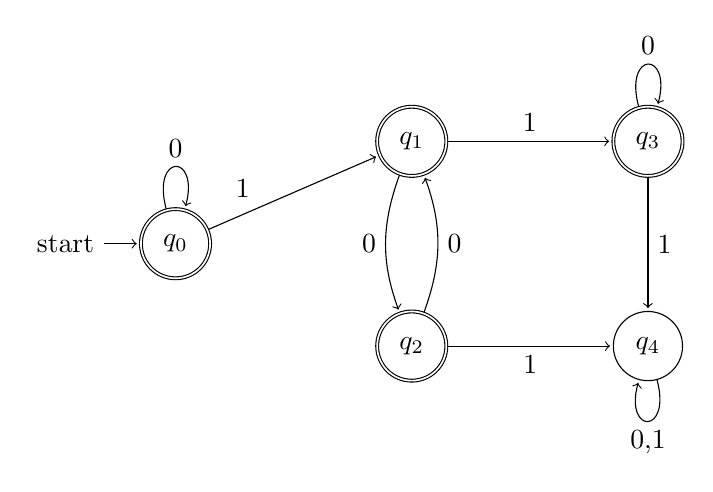
\begin{tikzpicture}[shorten >=1pt,node distance=3cm,on grid,auto,initial text=start]
  % 状态定义
  % q0: 起始，无1
  % q1: 有1个1，之后偶数个符号（0,2,4...）
  % q2: 有1个1，之后奇数个符号（1,3,5...）
  % q3: 有2个1，合法（间隔偶数）
  % q4: 陷阱（出现非法间隔或超过2个1）
  
  \node[state,initial,accepting] (q0) {$q_0$};
  \node[state,accepting] (q1) [right=of q0,yshift=1.3cm] {$q_1$};
  \node[state,accepting] (q2) [right=of q0,yshift=-1.3cm] {$q_2$};
  \node[state,accepting] (q3) [right=of q1] {$q_3$};
  \node[state] (q4) [right=of q2] {$q_4$};
  
  \path[->]
    % 从q0出发
    (q0) edge[loop above] node {0} ()
         edge node[above left,pos=0.3] {1} (q1)
    
    % q1和q2之间的偶奇计数循环（0来回切换）
    (q1) edge[bend right=20] node[left] {0} (q2)
         edge node[above] {1} (q3)  % 第二个1，间隔偶数，合法
    
    (q2) edge[bend right=20] node[right] {0} (q1)
         edge node[below] {1} (q4)  % 第二个1，间隔奇数，非法
    
    % q3状态（已有两个合法1）
    (q3) edge[loop above] node {0} ()
         edge node[right] {1} (q4)  % 第三个1，必与某1形成奇数间隔
    
    % 陷阱状态
    (q4) edge[loop below] node {0,1} ();
\end{tikzpicture}
\end{center}
\end{document}
